\section{Performance comparison} 
\label{sec:performance_comparison}

\begin{figure}
	\centering
	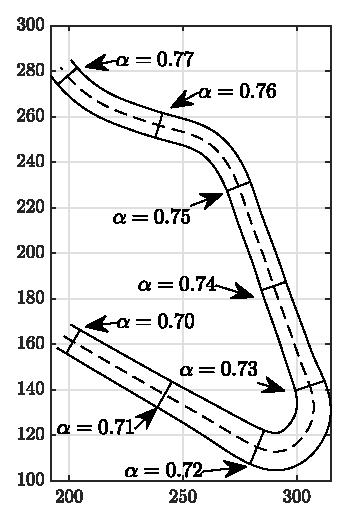
\includegraphics{Fig/track.eps}
	\caption{Sector of the Catalunya circuit considered in the analysis, corresponding to the curvilinear abscissa interval $\left[0.70, 0.77\right]$. Checkpoints are indicated by labels and are uniformly spaced by $\Delta\al=0.01$. This sector includes two distinct corners: a low-speed turn from $\al = 0.72$ to $\al = 0.73$, and a high-speed turn from $\al = 0.75$ to $\al = 0.76$, allowing for the evaluation of vehicle behavior across different dynamic scenarios.}
	\label{fig:track}
\end{figure}

\subsection{Robustified constraints comparison}
It is of interest to analyze how a robustified constraint---or a combination of the two described in Sections~\ref{sec:adherence_constraint} and~\ref{sec:stayontrack_constraint}---influences the driving style. This analysis compares the nominal trajectory, obtained without robustified constraints, with those resulting from a robustified stay-on-track constraint (denoted as SoT), a robustified adherence limit constraint (denoted as Adh), and a scenario where both constraints are robustified (denoted as SoT+Adh). All the optimization are obtained with the open-loop method described in Section~\ref{sec:open_loop_planning}, setting $H=4$, and $\ga^\textrm{SoT}=\ga^\textrm{Adh}=1.28$, corresponding to a 90\% probability of meeting both constraints. 

Figure~\ref{fig:ol_telemetries} presents the variation of four signals with respect to the nominal trajectory, for the three previously mentioned cases. The panels display the longitudinal speed $u$ (first panel), wheel steering angle $\delta$ (second panel), total longitudinal force $F_x$ (third panel), and lateral deviation of the center of mass from the track centerline $e$ (fourth panel). Except for the $u$ panel, each plot includes dashed black lines that indicate the sign of the nominal signal-whether it is positive, negative, or numerically zero. These sign indicators are represented as three distinct levels---high, zero, and low---corresponding to positive, zero, and negative values of the nominal signal, respectively. The levels are scaled appropriately in each plot to ensure clarity of visualization.

\begin{figure}
	\centering
	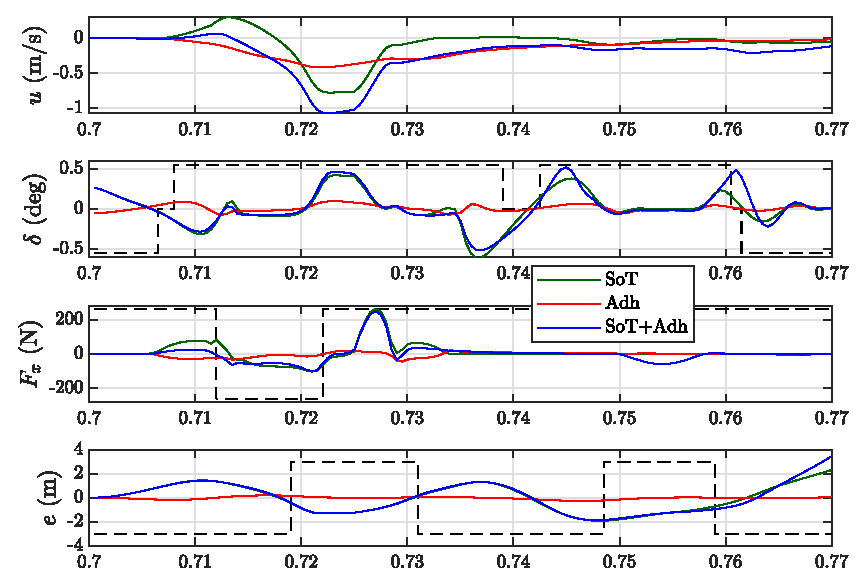
\includegraphics{Fig/ol_telemetries.eps}
	\caption{}
	\label{fig:ol_telemetries}
\end{figure}

From the first panel, it can be observed that all configurations maintain a lower mean value of the longitudinal speed compared to the nominal trajectory, resulting in an increased sector time. The two configurations incorporating the robustified stay-on-track constraint exhibit, as expected, a significantly altered CoM trajectory. This behavior explains the higher longitudinal speed observed around $\alpha = 0.71$, which is followed by a sharp reduction.

The second and fourth panels clearly show that the configurations with the robustified stay-on-track constraint tend to follow a path closer to the centerline. In particular, for most of the sector, the variation in lateral displacement and the lateral displacement $e$ itself exhibit opposite signs, indicating a corrective behavior of the steering angle $\de$ that pulls the vehicle toward the centerline.
